% !TeX program = pdflatex
\documentclass[twoside,a4paper,11pt]{article}
\usepackage{irrj2e}
\usepackage{booktabs}
\usepackage{amsmath}
\usepackage{lastpage}
\irrjheading{}{2026}{1--\pageref{LastPage}}{--}{--}{--}
\ShortHeadings{Selecting and Evaluating Multi-Hop Paragraph Evidence}{Mostafa}
\firstpageno{1}
\begin{document}
\title{Selecting Multi-Hop Evidence with Cached Paragraph Vectors: Structural Ranking and an Audit of Passage Sufficiency}
\author{\name Mohamed Mostafa \email mmsa12@gmail.com \\
\addr Independent Researcher}
\editor{Unassigned}
\maketitle

\begin{abstract}%
A multi-hop retriever must find paragraphs that support an answer together. Two individually relevant paragraphs can repeat the same fact, while a valid pair can differ from the one annotated by a benchmark. We study both problems. First, we compare lightweight structural ranking of cached paragraph vectors with independent dense ranking and Beam Retrieval. On 1,000 HotpotQA questions, a rule-based pair scorer increases exact supporting-pair recovery from 54.2\% to 79.1\%. A listwise multilayer perceptron reaches 84.1\%, compared with 96.5\% for Beam. Median selection time on 20 matched CPU requests is 11.15\,ms for the perceptron and 7.04\,s for Beam under the specified caching conditions. On 900 MuSiQue questions, structural features improve fixed-budget complete coverage from 45.2\% to 54.1\% in a matched CatBoost comparison. Second, two blinded AI reviewers judge 303 distinct passage sets returned by three baseline selectors on 150 questions. They identify both valid alternatives to annotated passages and annotated pairs with missing support. Both preserve the baseline ordering on each dataset. The audit measures how scoring affects the baselines; sufficiency of the full structural models remains unmeasured. The results quantify the cost and accuracy of paragraph selection and identify where exact recovery is an incomplete measure of its utility.
\end{abstract}
\begin{keywords}
multi-hop retrieval, paragraph ranking, evidence sufficiency, retrieval evaluation, inference latency
\end{keywords}

\section{Introduction}
Which other stadium shares a sports complex with the venue of the 1973 Pro Bowl? One passage records that the Pro Bowl took place at Arrowhead Stadium. A description of the Truman Sports Complex supplies the missing link: its two venues are Arrowhead and Kauffman. The question illustrates why relevance scores computed one paragraph at a time can be misleading. The second passage becomes particularly valuable once the first has identified Arrowhead. It also illustrates a different problem. In our HotpotQA audit, the two passages just described received zero under exact reference-pair recovery, although both reviewers could trace the answer through them.

The first problem is computational. A retriever can estimate interactions between the question and every growing evidence chain, as in Beam Retrieval \citep{beam}. This provides a strong accuracy reference, but repeated joint encoding adds query-time cost. An alternative is to encode paragraphs before the question arrives, then spend the online budget deciding which cached representations belong together. A shared entity, a directed title mention or two distinct comparison subjects are inexpensive signals of complementarity. Their usefulness depends on question type and on whether the candidate pool contains the necessary passages.

The second problem is measurement. Recovering an annotated set is objective and reproducible. A downstream reader instead needs evidence that establishes the answer, potentially through a different chain. An exact miss can therefore represent three different outcomes: a valid alternative chain, a single passage that already answers the question, or genuinely incomplete evidence. Conversely, a gold match may leave a qualification unstated. These cases have different implications for the design of a paragraph selector.

We ask three questions. (1) How much does explicit paragraph structure add beyond relevance under the same candidate budget and training conditions? (2) How do accuracy and request latency compare with joint encoding, and what changes when a selector must first discover candidates? (3) When independent readers evaluate returned text, how much does the measured advantage of a dense baseline over lexical retrieval change? The first two questions use the primary retrieval experiment. The third uses a separate diagnostic sample and a simpler title-link baseline for which item-level judgements are available. The shared dense baseline connects the experiments; their sample sizes, budgets and endpoints remain explicit throughout.

\section{Related work}
\paragraph{Multi-hop retrieval.}
HotpotQA introduced questions with sentence-level evidence annotations and bridge and comparison question types \citep{hotpot}. MuSiQue composes single-hop questions and applies constraints designed to make intermediate facts necessary \citep{musique}. Researchers have explored recurrent retrieval over linked paragraphs \citep{asai}, iterative multi-hop dense retrieval \citep{xiong}, and joint selection of a growing chain by beam search \citep{beam}. These approaches motivate our comparison: joint encoding can exploit detailed evidence interactions, while frozen document representations allow substantial computation to occur offline. Our contribution is an empirical comparison of the additional value of explicit structure, conditional on the supplied pool, and the consequences of the metric used to score that selection.

\paragraph{Evidence labels and evaluation.}
\citet{dire} study whether systems can succeed on multi-hop questions while bypassing intended reasoning steps. \citet{ni} show why unannotated contexts can be useful in multi-document QA. These observations imply that a single returned passage containing the answer deserves separate treatment from a newly discovered two-passage chain. A further distinction concerns the assessor. \citet{soboroff} explains why judgements generated by a language model can introduce systematic errors into IR evaluation. We release both AI readers' decisions, analyse each reader separately and report how much the observed disagreements could change each system contrast. This protocol measures sensitivity to the choice of assessment; it leaves human validity open.

\section{Paragraph selection}
\subsection{Representations and candidate sets}
For a question $q$, let $C_q$ be its candidate paragraphs and $G_q$ its annotated supporting set. Each paragraph has a title, body and frozen BGE embedding. With length-normalised vectors $u_q$ and $v_i$, the independent dense score is $r_i=u_q^\top v_i$. At budget two, selecting the highest-scoring pair under
\[
 s_0(i,j\mid q)=r_i+r_j,\qquad i\ne j,
\]
is equivalent to taking the two highest individual scores. This baseline can select two paragraphs that cover the same entity or topic. It assigns no additional value to a paragraph that completes a specific relation with its partner.

\subsection{Directed links, comparison slots and gated matching}
The rule-based selector starts from $s_0$ and ranks unordered paragraph pairs. It treats a title mention as directional: one paragraph can name the subject of a second paragraph even when the reverse mention is absent. For a bridge question, the scorer rewards an eligible first paragraph whose text identifies the partner, together with question and sentence cues for the requested relation. For a comparison question, separate slots reward coverage of distinct question subjects. This discourages two high-similarity paragraphs about the same subject from filling both slots.

A logistic classifier over hashed question n-grams chooses the question type. A second decision uses the classifier's uncalibrated bridge score. At the fixed cutoff of 0.90, the scorer enables a wider first-hop shortlist and relaxed title matching. The final rule also rewards coverage of weighted question terms across the pair. The gate controls when to apply the more permissive matching rule. The numerical cutoff should therefore be interpreted as an implementation setting, rather than a calibrated probability that the question is a bridge question. The rules and bonuses were fixed before selection of the final HotpotQA evaluation sample.

\subsection{Matched feature ablation and learned ranking}
To isolate structure from a stronger relevance model, we compare two CatBoost models trained with the same settings. Both receive BGE cosine, BM25, word and character TF--IDF, and corresponding rank features. The structured model adds question-to-title matches, directed links to relevant neighbours, graph degree and inter-paragraph similarity. The difference between these two models is the primary structural ablation. Comparing the full rule scorer with BGE answers a broader question because that contrast changes several components at once.

On HotpotQA we score every unordered candidate pair, giving 45 alternatives for ten candidates. A listwise linear model and a one-hidden-layer multilayer perceptron (MLP) were also explored. On MuSiQue we score individual passages with features calculated over the whole candidate pool, then rank the passages. This formulation accommodates questions with more than two supporting paragraphs. The two-slot HotpotQA heuristic has no directly comparable result in that setting.

\section{Experimental design and metrics}
\subsection{Main retrieval experiment}
The final HotpotQA Distractor sample contains 1,000 official validation questions with ten distinct candidate titles and two supporting paragraphs. Selection excluded 5,820 question IDs used in previous experiments in the project. The MuSiQue-Ans experiment uses 900 development questions with 20 candidates and two to four annotated supports. These questions had been used in earlier experiments, which makes MuSiQue a secondary evaluation. Each dataset supplies a separate 1,200-question training set for supervised parameters or feature statistics and 400 questions available for tuning. Training is dataset-specific. We report seed 42 and examine variation across seeds 13, 42 and 97 where available.

For a returned set $S_q(k)$ of size $k$, exact match is $\mathbf{1}\{S_q(k)=G_q\}$. On HotpotQA the budget is two. On MuSiQue, matched-count exact match uses $k=|G_q|$, an oracle quantity. The operational alternative fixes $k=4$ and measures complete coverage, $\mathbf{1}\{G_q\subseteq S_q(4)\}$. A two-support question can receive full credit for a four-passage set under coverage. The two MuSiQue columns therefore answer different questions. All results concern paragraph selection. Neither answer generation nor sentence-level HotpotQA scoring is part of the main experiment.

Beam accuracy uses the released predictions filtered to the same evaluation IDs. Runtime uses the released DeBERTa-large width-one checkpoint on a matched subset. Reported intervals use 5,000 paired bootstrap resamples of questions. Intervals are descriptive and unadjusted for multiple comparisons.

\subsection{Audit design}
A second experiment samples 50 HotpotQA validation questions from 7,405 eligible examples and 100 two-hop MuSiQue development questions from 1,252 eligible examples. Sorting by ID precedes seeded uniform sampling. The HotpotQA sample contains 42 bridge and eight comparison questions. Both datasets use a two-passage budget. Samples come from the same development resources used in the primary study; we make no claim of disjointness between studies.

Three selectors enter the audit: candidate-pool BM25, independent BGE, and an exploratory BGE pair scorer that adds 0.05 to the sum of the two similarities if either body mentions the other's normalised full title. This last method omits the question-type classifier, relaxed matching, comparison slots and keyword bonus. It tests the simplest connection between paragraphs on the audit sample. It cannot stand in for the full gated scorer or the learned rankers.

Each question--set combination is assessed once per reviewer even when multiple systems return it. The 150 HotpotQA outputs yield 105 distinct sets, and the 300 MuSiQue outputs yield 198. Two fresh AI sessions using the same assistant configuration receive independently shuffled worksheets with the question, proposed answer, titles and passages. They receive no system or gold labels, and work without external lookup or the other session's decisions. Readers may use elementary arithmetic and ordinary language interpretation. They classify each pair as \emph{single} (one passage suffices), \emph{joint} (both are required and together suffice), \emph{insufficient} or \emph{indeterminate}. Positive decisions require quoted text; joint decisions require excerpts from both passages. We checked that each positive excerpt occurs in the supplied evidence. This check establishes textual provenance only.

\subsection{Paired comparison}
Let $h_r(q,m)$ equal one when reader $r$ judges the set from method $m$ to have single or joint support, and zero otherwise. For two methods $a,b$, the audited gap is the mean of $h_r(q,a)-h_r(q,b)$. We compare it with the gold gap on the same questions by resampling the paired difference of differences. Each reader is analysed separately. Repeated outputs retain a shared label in all contrasts. The bootstrap varies questions and holds reader decisions fixed; it measures sampling uncertainty conditional on those decisions.

\section{Retrieval results}
\begin{table}[t]
\centering\small
\begin{tabular}{lrrr}\toprule
& HotpotQA & \multicolumn{2}{c}{MuSiQue}\\
\cmidrule(lr){3-4}
Method & EM at 2 & EM at $|G_q|$ & Coverage at 4\\\midrule
BM25 &19.8&5.0&---\\
MiniLM &17.0&1.2&---\\
BGE-small &54.2&13.0&26.9\\
Gated slots + keywords &79.1&---&---\\
CatBoost, relevance &61.3&26.3&45.2\\
CatBoost, relevance + structure &83.7&34.6&54.1\\
Listwise MLP, relevance + structure &84.1&31.6&49.9\\
Beam Retrieval (released predictions) &96.5&79.2&---\\\bottomrule
\end{tabular}
\caption{Paragraph selection in supplied pools. Values are percentages on 1,000 HotpotQA and 900 MuSiQue questions. A dash means no value is reported here. Matched-count MuSiQue evaluation supplies the gold support count.}\label{tab:primary}
\end{table}
Table~\ref{tab:primary} gives the main result. Structural features raise HotpotQA exact match from 61.3\% to 83.7\% for matched CatBoost models, a gain of 22.4 percentage points (95\% interval 19.5 to 25.3). On MuSiQue they raise fixed-budget complete coverage from 45.2\% to 54.1\%, a gain of 8.9 points (6.2 to 11.7). The sign carries across the datasets and across their two ranking formulations. The results do not identify a single structural feature as the cause; the matched ablation changes the feature group.

On HotpotQA the fixed gated scorer with keywords gains 24.9 points over independent BGE (22.1 to 27.9). Adding keyword coverage contributes 1.6 points on the final sample (0.6 to 2.6). The listwise MLP and structured CatBoost are close on HotpotQA, whereas the structured tree model has the higher fixed-budget MuSiQue coverage. Across three seeds, HotpotQA MLP exact match ranges from 84.1 to 84.7\%, and structured CatBoost from 83.0 to 83.7\%. Structured CatBoost reaches 53.0 to 54.1\% on fixed-budget MuSiQue. We have little basis for attributing special significance to the 0.4-point difference between the two HotpotQA models at seed 42.

Compression and pair structure address different costs. Scalar int8 quantisation followed by dequantised cosine preserves aggregate HotpotQA BGE exact match at 54.2\% and changes MuSiQue matched-count exact match by 0.1 points. PCA to 64 or 128 dimensions reduces accuracy on both datasets. These experiments concern retrieval quality. They do not establish end-to-end memory or latency savings.

\subsection{CPU latency under matched conditions}
Twenty preselected HotpotQA requests were timed sequentially on a MacBook Pro with an Apple M1 and four PyTorch threads. The candidate paragraphs were matched across methods. Cached selectors preload paragraph vectors and title links; the rule scorer also preloads paragraph keyword metadata. Learned scorers recompute sparse features from candidate text. Beam tokenises candidates and encodes growing chains, using a 512-token cap and two hops. Its local selections matched the released predictions on all 20 timed requests. Timing includes query processing and selection and excludes model loading, candidate discovery and answer generation.

\begin{table}[htbp]\centering\small
\begin{tabular}{lrrr}\toprule
Selector & EM (\%) & Median (ms) & 95th percentile (ms)\\\midrule
Gated slots + keywords &79.1&10.11&11.36\\
Structured CatBoost &83.7&11.56&13.02\\
Structured listwise MLP &84.1&11.15&12.79\\
Beam Retrieval &96.5&7,036&9,322\\\bottomrule
\end{tabular}
\caption{Selection latency on 20 matched CPU requests. Accuracy uses the larger 1,000-question sample. The 95th percentile is descriptive for this small timing set.}\label{tab:time}\end{table}

At seed 42 the MLP gives up 12.4 exact-match points to Beam. The ratio of medians in Table~\ref{tab:time} is approximately 631. Much of this difference has a concrete explanation: the cached system reuses paragraph encoding across requests, while the tested Beam implementation encodes each chain in query context. The comparison is relevant to recurring queries over stable paragraphs on a CPU. Cold-cache operation, an optimised Beam runtime, hardware acceleration and the cost of maintaining the index can change the trade-off.

\subsection{When candidates must first be discovered}
Supplied-pool selection removes a distinct source of failure. To estimate its effect, a separate experiment deduplicated passages from the training and final HotpotQA pools into a shared index of 24,955 paragraphs. The index includes the labelled passages by construction. Evaluation questions and gold labels were excluded from candidate-feature construction. Both gold passages reached the top ten on 74.3\% of queries for BGE and 76.7\% for BGE plus BM25 reciprocal rank fusion. End-to-end exact match after reranking those ten with the gated scorer was 61.5\% and 61.8\%, respectively. At depth 50, fusion raised complete candidate coverage to 90.8\%; the greater depth also increases the number of pairs to examine.

The 2.4-point improvement in top-ten coverage translated into only 0.3 points of final exact match. Dividing end-to-end recovery by candidate coverage gives approximate conditional success of 82.8\% for BGE candidates and 80.6\% for fused candidates; these ratios use the reported rounded rates. Candidate recall bounds what selection can recover, and changing the candidate generator also changes the distractors the selector encounters. These observations apply to this constructed index rather than full Wikipedia search.

\section{Does annotated recovery reflect sufficient evidence?}
The preceding experiments evaluate whether structural ranking recovers a benchmark's reference paragraphs. A method that uses title links might be particularly good at reproducing the annotation path. To examine what the metric credits, Table~\ref{tab:audit} compares exact recovery with two readers' assessments for the three audit selectors. Absolute results differ from Table~\ref{tab:primary} because the audit samples were drawn separately and the MuSiQue audit includes only two-hop questions.

\begin{table}[htbp]\centering\small
\begin{tabular}{llrrr}\toprule
Dataset & Method & Gold pair & Reader A & Reader B\\\midrule
HotpotQA ($n=50$)&BM25&9&12&13\\
&BGE&24&24&26\\
&BGE + title link&29&27&30\\\addlinespace
MuSiQue ($n=100$)&BM25&13&11&11\\
&BGE&26&25&26\\
&BGE + title link&27&26&27\\\bottomrule
\end{tabular}
\caption{Questions credited by exact reference recovery or by each blinded AI reader. Each reader credits evidence sufficient in one or both passages.}\label{tab:audit}
\end{table}

On HotpotQA, BGE leads BM25 by 30 percentage points under gold scoring. The readers reduce the gap to 24 and 26 points. The paired changes are $-6$ points (95\% interval $-16$ to $+2$) and $-4$ points ($-14$ to $+6$). On MuSiQue the 13-point gold gap becomes 14 and 15 points. The paired changes are $+1$ point ($-4$ to $+6$) and $+2$ points ($-3$ to $+7$). Each interval includes zero (Figure~\ref{fig:tradeoff}, right). The ordering of all three baseline selectors was preserved for both readers on both datasets. These samples establish neither equivalence of the evaluation criteria nor the ranking of the full structural models under sufficiency scoring.

\begin{figure}[htbp]\centering
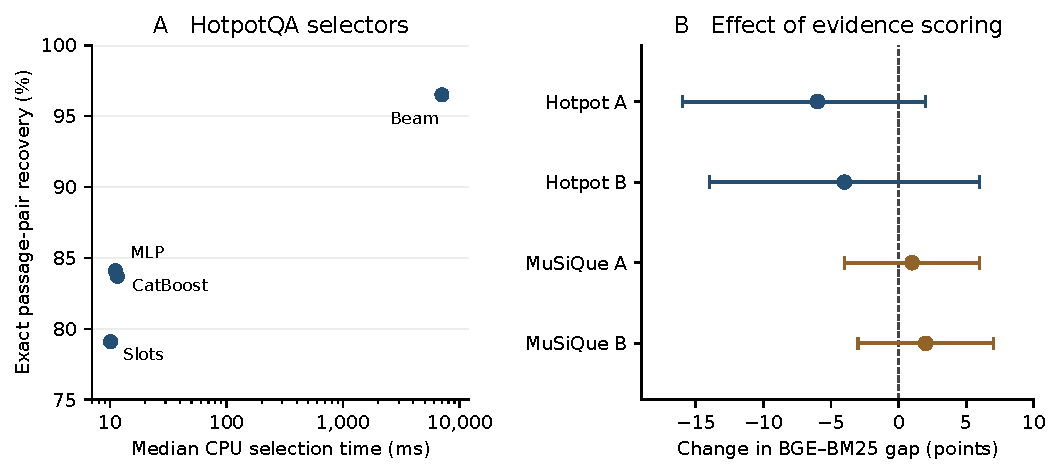
\includegraphics[width=\linewidth]{figures/selection-audit.pdf}
\caption{Two measurements of paragraph selection. Left: HotpotQA accuracy for the main selectors against median warm-cache CPU latency (log scale). Right: change in the BGE minus BM25 gap when annotated-pair recovery is replaced by each AI reader's sufficiency judgement. Bars show paired 95\% bootstrap intervals. The panels use the different samples described in the text.}\label{fig:tradeoff}
\end{figure}

\subsection{What net scores conceal}
On MuSiQue, Reader B credits BGE on 26 questions under either metric. Four non-gold sets gain credit: two single-passage answers and two alternative joint answers. Four gold sets lose credit. Reader A also credits two new single and two new joint sets but rejects five gold sets. Both readers add three single-passage successes for BM25 and reject five of its gold pairs. The aggregate score alone hides which questions the system serves well.

The Pro Bowl question illustrates an alternative joint answer. A question asking for the other title of Shakespeare's \emph{Twelfth Night} illustrates a different outcome: the play's own paragraph supplies \emph{What You Will} directly. BM25 paired it with a passage about the film adaptation, missing the gold set. Crediting this pair is appropriate for passage sufficiency but supplies no evidence of combining two facts. In another case the two gold paragraphs identify the states of origin of two bands. Neither paragraph establishes which state is larger. Both readers reject the reference under the passage-only rule. A task permitting geographic world knowledge could reasonably assign a different label.

The reviewers agree on 102 of 105 HotpotQA sets and 197 of 198 MuSiQue sets. The same counts hold for binary and four-way decisions. Binary Cohen's $\kappa$ is 0.94 and 0.98, respectively. Allowing every dispute to take either reader's binary value, while assigning the same decision wherever a set is shared, leaves a BGE advantage of 12--13 questions over BM25 on HotpotQA and 14--15 on MuSiQue. The bounds cover observed disputes only.

One reviewer identified a question--answer mismatch. A post hoc screen for questions asking what or which year, paired with an answer lacking a four-digit year, identified one of 150 questions. The proposed answer to this MuSiQue question is November 5. All three systems missed the reference pair and both readers rejected every returned set. Excluding the item preserved the success counts and ordering over the remaining 99 questions. Other forms of mismatch remain possible.

\section{Discussion}
\paragraph{When does paragraph structure pay off?}
The matched CatBoost comparison gives the cleanest answer in this study. Structural features improve recovery on both datasets, including fixed-budget coverage on MuSiQue. The rule experiment shows how much of the HotpotQA gain is available without a trained pair ranker. In contrast, the simple title bonus in the diagnostic experiment adds five gold matches in aggregate on HotpotQA and one on MuSiQue. These experiments use different samples, so their difference is not a component ablation. They motivate a direct examination of which questions benefit from gated matching, subject coverage and learned interactions.

\paragraph{Where does evidence go missing?}
The two studies identify three distinct points of failure. Discovery can omit a necessary paragraph. Selection can choose redundant or disconnected passages from an adequate pool. Scoring can reject a sufficient alternative or accept a gold pair that relies on outside knowledge. Measuring the discovery ceiling and ablating the ranker's structural features address the first two effects. A blinded audit exposes the third. The measured 22.4-point structural gain on HotpotQA cannot be interpreted as 22.4 more answerable questions per hundred. That interpretation would require sufficiency judgements on the two CatBoost variants' actual outputs.

\paragraph{What would distinguish the strongest systems?}
For recovery of the annotated evidence path, Beam is the strongest system measured. For stable documents, a warm cache and a CPU selection budget near the measured times, the MLP offers a different operating point. To distinguish these systems on reader utility, a follow-up should pool the actual Beam, MLP and gated-scorer outputs for the same questions, retain examples on which the systems agree, and blind human readers to system identity. Sampling both reader agreements and disputes would also test for systematic errors that two related AI assessors share.

\section{Limitations}
The primary HotpotQA split excluded previously used IDs but shares its task design with development work. The 900 MuSiQue questions had already been explored. The discovery index includes supporting passages by construction and is much smaller than an open-domain corpus. Early explorations of attention across cached paragraph vectors motivated the structural comparison. No score for paragraph self-attention was available on the final matched splits. The listwise MLP in the main table scores engineered features and should not be interpreted as that attention model.

Timing covers 20 requests on one CPU. Only the timing subset was rerun locally with Beam; the larger accuracy comparison uses its released predictions. The audit's reviewers share a model family and a proposed answer, and may share confirmation biases. Checking their quotations establishes provenance, while human validity remains open. The primary result tables report the archived retrieval experiment. The accompanying public implementation and labels reproduce the separate audit. Fully reproducing training of the original structural rankers requires the corresponding original experimental assets.

\section{Conclusion}
A paragraph's value to a multi-hop question depends on what the other paragraphs establish. Cross-paragraph features improved annotated evidence recovery in matched ablations, and cached selection exposed a sizeable CPU accuracy--latency trade-off. Reviewing the returned text revealed sufficient alternatives and incomplete reference pairs, even as the baseline rankings held. Candidate coverage, conditional ranking accuracy and answer support therefore describe different properties of a paragraph retrieval system. Reporting all three makes it possible to identify which part merits further engineering.

\acks{The experiments use HotpotQA, MuSiQue and the released Beam Retrieval predictions and model. Generative AI assisted with experimental code, analysis and manuscript drafting. Two AI sessions supplied the audit judgements.}
% Author to verify funding and competing-interest disclosures before submission.
\appendix
\section{Reproducing the audit}
The public repository contains sampling and retrieval scripts, system outputs, the review rubric, both readers' labels, and code for agreement, paired intervals and dispute bounds.\footnote{\url{https://github.com/mmsa/multihop-evidence-audit/tree/e6eff5f64386cf992fb8d99d4b652357043f0d2a}} The audit uses seeds 20261126 and 20261127 for HotpotQA and MuSiQue sampling, respectively. HotpotQA is scored by title in candidate pools with unique titles. MuSiQue is scored by passage index because titles can repeat. Each audit encoder input contains a prefixed question or a title and paragraph body, with normalised CLS pooling and 512-token truncation. BM25 uses candidate-pool document frequencies with $k_1=1.2$ and $b=0.75$.

Let $F^+$ count non-gold predictions credited by a reader and $F^-$ count gold predictions judged insufficient or indeterminate. On $n$ questions the difference between judged sufficiency and exact recovery is $(F^+-F^-)/n$. The gap between systems changes only when their net corrections differ. Whenever two systems return the same set for a question, that question contributes zero to their paired difference under either criterion. Deduplicating assessments within a question therefore preserves the question-level denominator.

\bibliography{references}
\end{document}
